
% how to compile: platex xxx.tex ; dvipdfmx xxx.dvi

\documentclass[a4paper]{jarticle}

%--余白の設定
\setlength{\topmargin}{20mm}
\addtolength{\topmargin}{-1in}
\setlength{\oddsidemargin}{20mm}
\addtolength{\oddsidemargin}{-1in}
\setlength{\evensidemargin}{15mm}
\addtolength{\evensidemargin}{-1in}
\setlength{\textwidth}{170mm}
\setlength{\textheight}{254mm}
\setlength{\headsep}{0mm}
\setlength{\headheight}{0mm}
\setlength{\topskip}{0mm}
\renewcommand{\baselinestretch}{0.4}
%--ハイバーリンクを可能にするパッケージ
\usepackage[dvipdfmx,%
 bookmarks=true,%
 bookmarksnumbered=true,%
 colorlinks=true,%
 setpagesize=false,%
 pdftitle={msortf},%
 pdfauthor={BMRC},%
 pdfkeywords={TeX; dvipdfmx; hyperref; color;}]{hyperref}
\usepackage{graphicx}
\usepackage{multirow}  
\begin{document}

\setlength{\baselineskip}{4mm}

\section*{msortf (sort by specific column) command}
Sort records according to the field defined at \emph{f=} parameter.\\
This commands uses quicksort algorithm and it is not a stable sort. Original order is saved for rows with same key value.  \\

\subsection*{Format}
msortf f=  
[\href{run:option.pdf}{tmpPath=}] 
[\href{run:option.pdf}{-nfn}] 
[\href{run:option.pdf}{-nfno}] 
[\href{run:option.pdf}{-x}] 
[\href{run:option.pdf}{i=}] 
[\href{run:option.pdf}{o=}] 
[--help]\\

\subsection*{Parameters}
\begin{table}[htbp]
%\begin{center}
{\small
\begin{tabular}{ll}
\verb|f=|    & Field name(s) [\%n$|$\%r$|$\%nr]【required parameter】\\
& Specify the column name where record values will be sorted accordingly. \\
& Records are sorted as character string by default when field name is specified.\\
& Specify "\%n" after the field name i.e. \emph{f = item name\%n} to sort by numerical values.\\
& Sort fields in descending order according to numerical values using \emph{f = item name\%r} and according to character strings using \emph{f = item name\%nr} respectively.  \\
& NULL value in the data is treated as a value less than any other numeric or string character.\\
& Sort on multiple columns by specifying the field names separated by comma (,) listed according to the priority. \\
& Note: \emph{\% n} only works on numerical values and will result in undefined behavior when sorting character strings. \\
\end{tabular} 
}
\end{table} 

\subsection*{Option}
\begin{table}[htbp]
%\begin{center}
{\small
\begin{tabular}{ll}
\end{tabular} 
}
\end{table} 

\subsection*{Examples}
\subsubsection*{Example 1 Sort by item and date.
}
\renewcommand{\tablename}{table }

\begin{verbatim}
------------------------------------------------
# Input file (dat.csv)
item,date,quantity,price
B,20081201,4,40
A,20081201,10,200
A,20081201,10,100
B,20081203,5,50
B,20081201,2,500
A,20081201,3,300

$ msortf f=item,date i=dat.csv o=rsl.csv

# Output file (rsl.csv)
item,date,quantity,price
A,20081201,10,200
A,20081201,10,100
A,20081201,3,300
B,20081201,4,40
B,20081201,2,500
B,20081203,5,50
------------------------------------------------
\end{verbatim}

\subsubsection*{Example 2 Sort quantity in descending order and price in ascending order.
}

\begin{verbatim}
------------------------------------------------
# Input file (dat.csv)
item,date,quantity,price
B,20081201,4,40
A,20081201,10,200
A,20081201,10,100
B,20081203,5,50
B,20081201,2,500
A,20081201,3,300

$ msortf f=quantity%nr,price%n i=dat.csv o=rsl.csv

# Output file (rsl.csv)
item,date,quantity,price
A,20081201,10,100
A,20081201,10,200
B,20081203,5,50
B,20081201,4,40
A,20081201,3,300
B,20081201,2,500
------------------------------------------------
\end{verbatim}

\subsection*{Advanced parameters}
\begin{table}[htbp]
%\begin{center}
{\small
\begin{tabular}{ll}
\verb|pways=|    & Merge multiple files simultaneously ([2-100]:default 32)【Optional】\\
& Specify  number of files to merge at a time while sorting multiple files. \\
\verb|blocks=|   & Number of buffer block ([1-1000]: default 100 1blk=400KB)【Optional】\\
& Specify memory size limit in the block size when sorting in memory.\\
& Maximum size for 1 block is × 4. Default = 400KB. \\
\verb|maxlines=| & Row fetch limit of memory sort ([100-10,000,000]: 500,000 defaults)【Optional】\\
& Specify the maximum number of records sorted at once in memory.\\
& Set -block limit and -maxlines limit depending on the average size of record in the data.\\
\verb|threadCnt=| & Number of threads to use when sorting in memory ([1-50] Default: 8)【Optional】\\
& Specify the number of threads for sorting through multi-threading function. \\
\end{tabular} 
}
\end{table} 

\subsection*{Notes on sorting order of CSV special characters}
CSV is a delimited at a format that commonly employs ASCII character set. The data fields/columns are separated by comma character. Comma and double quotes is treated as special characters in CSV is enclosed in double quotes. msortf interprets and sorts CSV special characters (e.g. comma and double quotes) differently than the sort command in UNIX. 
For example, the values in the first column (f1) from the first row onwards are represented by the following ASCII characters: 
a -> (0x61)
null -> (0x00)
space -> (0x20)
+ -> (0x2b)
- -> (0x2d)
, -> (0x2c) 
" -> (0x22)

For ease of illustrating fields in the first column (f1), "x" is populated in the second column (f2) for all records as follows. \\

\begin{verbatim}
------------------------------------------------
f1,f2
a,x
,x
 ,x
+,x
-,x
",",x
"""",x
------------------------------------------------
\end{verbatim}

The statement \verb|msortf f = f1| sorts the data as follows.  The records are sorted by f1 according to ASCII characters in CSV format (null, space, double quotation, +, comma,-, a). 

\begin{verbatim}
------------------------------------------------
f1,f2
,x
 ,x
"""",x
+,x
",",x
-,x
a,x
------------------------------------------------
\end{verbatim}

\subsection*{Benchmark Test}
The benchmark test described here shows the performance of msort and msortf. 
The input data consist of 6 fields and all data values are uniform random numbers. \\

\begin{verbatim}
------------------------------------------------
key,fld1,fld2,fld3,fld4,fldn
95547922,162,159,192,118,74
81438069,138,157,155,122,58
26885062,129,199,133,198,75
32651684,180,107,123,170,-14
10245631,164,103,159,154,-63
15145156,182,191,175,107,-60
29254245,188,185,129,124,5
85423170,116,164,175,113,57
55155879,105,163,195,167,25
66997216,195,139,195,113,39
.
.
------------------------------------------------
\end{verbatim}

\subsection*{Compare number of key types and values}
The sample data size is 1 million, the following table shows the results according to variation in types of key values at 2,10,100,1000,10000.
Data in the "random number" column is generated using the maximum limit of the random number as key. 
Data is sorted according to the values in "random number ascending / descending order" column before the benchmark test. 
The comparison table shows the processing results of msort, MUSASHI xtsort command, and UNIX sort command against the msortf command.
The sort command sort one or more sort keys extracted from each line of input, whereas "sort -k1" sorts data on the first column. 
The last 3 rows of the table show the result of  msortf, xtsort and sort sorted on numeric value stored in the first key field.
※ Input data size: about 28MB.\\
※ Unit: seconds. Measurement in real time from beginning to end of program using the time command. \\
※ Environment: iMac, Mac OS X 10.5 Leopard, 2.8GHz Intel Core 2 Duo, 4GB memory \\

\begin{table}[h]
\begin{center}
\caption{The comparison of the number of the types and the condition of the value of key item}
 \begin{tabular}{cccccccccc}
\hline
No. & command & 2types & 10 types & 100 types & 1000 types & 10000 types & random number & random number ascending order & random number descending order\\
\hline
(1) & msort & 1.24 & 1.12 & 2.07 & 1.11 & 1.12 & 1.78 & 0.82 & 0.67\\
(2)	& msortf k=key & 1.14 & 1.02 & 2.42 & 1.21 & 1.16 & 2.68 & 1.08 & 0.96\\
(3)	& xtsort -k key & 1.74 & 1.55 & 3.06 & 1.53 & 1.52 & 3.04 & 1.06 & 1.37\\
(4)	& sort & 42.36 & 41.91 & 40.26 & 38.99 & 37.26 & 33.33 & 15.82 & 15.30\\
(5)	& sort -k1 & 42.56 & 42.30 & 40.63 & 39.92 & 37.81 & 33.67 & 15.95 & 15.52\\
(6)	& msortf k=key\%n & 1.76 & 1.85 & 2.30 & 2.52 & 2.85 & 3.06 & 1.53 & 1.61\\
(7)	& xtsort -k key\%n & 4.03 & 4.53 & 5.48 & 5.88 & 6.02 & 5.95 & 3.23 & 3.19\\
(8)	& sort -k1 -n & 41.63 & 36.41 & 29.15 & 22.16 & 14.92 & 2.26 & 1.37 & 1.37\\
\hline
 \end{tabular}
\end{center}
\end{table}
\newpage
The results of (1),(2),(3) are shown in the graph below. \\
\begin{figure}[!h]
\begin{center}
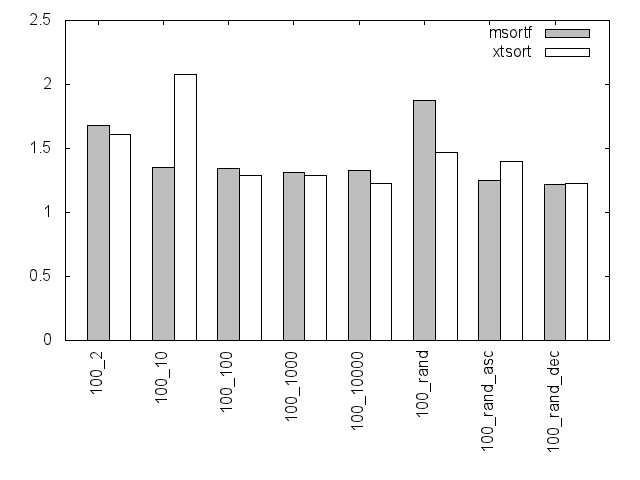
\includegraphics[width=10cm,bb=0 0 400 200]{./img/key.png}
\end{center}
\caption{Compare sort results on character data with msort, msortf, xtsort based on number of key types. (x-axis: number of the key type, y-axis: seconds)}
\end{figure}

The following graph show the results of (6),(7)\\
\begin{figure}[!h]
\begin{center}
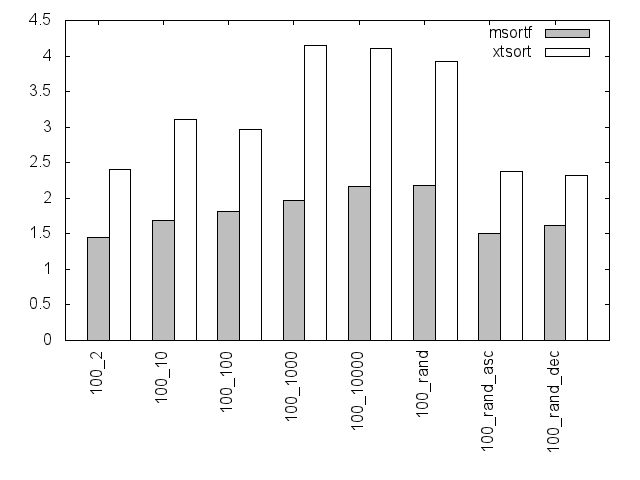
\includegraphics[width=10cm,bb=0 0 400 200]{./img/num.png}
\end{center}
\caption{Compare sort results on numeric data with msort, msortf, xtsort based on number of key types. (x-axis: number of the key type, y-axis: seconds)}
\end{figure}

\newpage
As shown in the benchmark test, msort is 1.5 times faster than MUSASHI xtsort. Even though both commands uses the same quicksort algorithm, msort leverages on multi-threaded sort processing using kgmod which runs 1.5 times faster. 
msort performs better than msortf on data with irregular keys that is sorted beforehand, as sorting is done by line without dividing the data. Thus, small variation in key types for the first item makes it difficult for comparison as the correlation magnitude has not been established.  The need for comparison created a higher overhead. 
In addition, the msort command process faster than msortf on data with multiple columns.  However, using msort to sort the key field of input data for other commands may yield different results if the command is executed incorrectly. For more information, refer to msort command. \\

The results also show that msortf is two times more efficient than xtsort in sorting numeric fields.
Next, the sorting speed is compared amongst msortf, msort, and xtsort on data with a sample size of 10 million with 2 to 100 different key values. The results are shown as follows: \\

\begin{figure}[!h]
\begin{center}
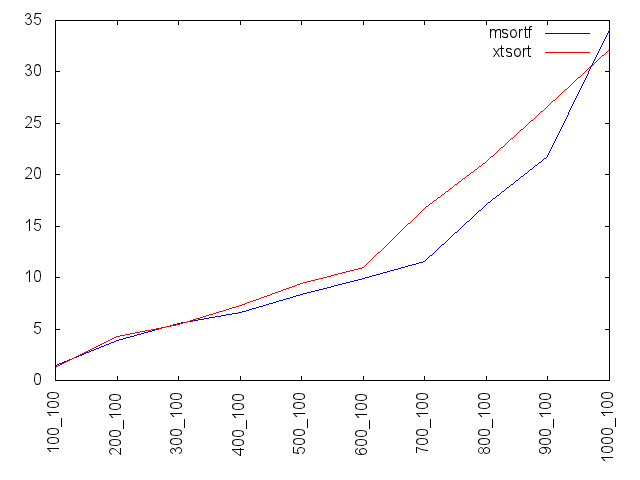
\includegraphics[width=10cm,bb=0 0 400 200]{./img/line_100.png}
\end{center}
\caption{Sorting results with the 100 number of key types (x-axis: number of records, y-axis: seconds)}
\end{figure}

\begin{figure}[!h]
\begin{center}
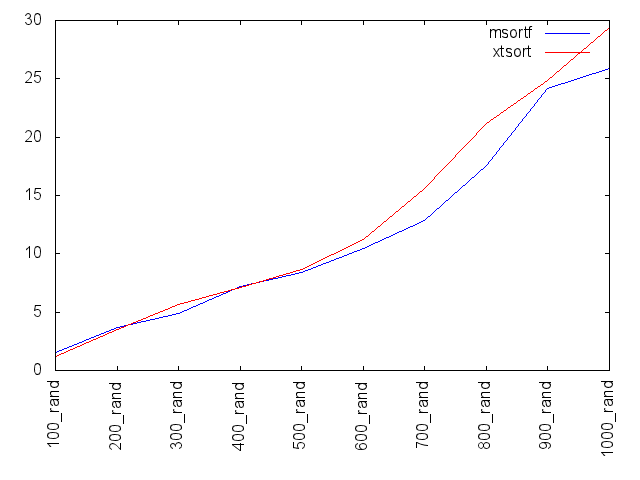
\includegraphics[width=10cm,bb=0 0 400 200]{./img/line_rand.png}
\end{center}
\caption{Sorting results with key types using random number (maximum) (x-axis: number of records, y-axis: seconds)}
\end{figure}

\subsection*{Related Command}
\noindent
\href{run:msort.pdf}{msort}: reorder of records based on field value\\

\end{document}
